\section{ВВЕДЕНИЕ В МАШИННОЕ ОБУЧЕНИЕ}
Обработка естественного языка является крайне тяжелой задачей для моделирования стандартными методами. Машинное обучение позволяет решать задачи на основе статистических наблюдений из данных без явной алгоритмизации решения задачи. Недавние прорывы в области обработки естественного языка показывают, что методами машинного обучения можно частично или сполна выполнять многие человеческие задачи, например, краткое изложение текста, написание кода, общение с собеседником и другие, добиться результатов распознавания речи сопоставимых с результатами человека \cite{human-wer,whisper}.

Основным аспектом машинного обучения является модель машинного обучения, иногда называемой искусственной нейронной сетью (ИНС), созданной по подобию биологических нейронных сетей, или просто нейронной сетью. Модель машинного обучения -- описание сети, математическая модель, часто представляемая в виде графа, нацеленная на решение задачи прогнозирования на основе обучающей выборки данных. Методами настройки параметров модели под конкретную задачу называют методами обучения. Такими методами являются: обучение с учителем, обучение без учителя и обучение с подкреплением. Каждый метод имеет свои особенности и применяется в зависимости от ситуации. Например, обычно обучение с учителем применяется в тех случаях, когда обучающий набор данных размечен на основе некоторых критериев. Такие задачи обычно являются задачами классификации, когда каждый экземпляр выборки имеет один или больше собственный класс. Такой подход имеет ограничения: как правило количество размеченных данных значительно меньше общего количество данных. В ситуации, когда данные не размечены, применяется обучение без учителя. Благодаря такому подходу, можно обучить модель делить данные на кластеры, генерировать текст, изображения и т.д. Когда модели приходится принимать решения как интеллектуальный агент в условиях данной ей среды и соотвествующих откликов среды на решения, применяется метод обучения с подкреплением. Для построения мощных современных цифровых ассистенов могут использоваться все три подхода к обучению моделей, используя модели, полученных конкретным методом, в качестве промежуточных или вспомогательных, для обучения конечной модели \cite{state-of-gpt}.

Устройство простой ИНС можно описать как взвешенный набор узлов, разделенный на слои, соединенные между собой активационными функциями $\varphi$. При построении модели ИНС в качестве активационных функций часто используется одна из следующих функций:
\begin{enumerate}
    \item Гиперболический тангенс:
          \begin{equation}
              \varphi(z) = \frac{e^{2z}-1}{e^{2z}+1}.
          \end{equation}
    \item Функция ReLU:
          \begin{equation}
              \varphi(z) = \max(0, z).
              \label{relu}
          \end{equation}
    \item Функция GELU:
          \begin{equation}
              \varphi(z) = \frac{1}{2}z\Big[1+\text{erf}({z}/\sqrt{2})\Big].
              \label{gelu}
          \end{equation}
    \item Логистическая функция (сигмоида):
          \begin{equation}
              \varphi(z) = \frac{1}{1+e^{-z}}.
          \end{equation}
    \item Многопеременная логистическая функция (softmax):
          \begin{equation}
              \varphi(z)_i = \frac{e^{z_i}}{\sum_{i=1}^{K}e^{z_j}}.
          \end{equation}
\end{enumerate}

Архитектуры ИНС могут сильно отличаться друг от друга в зависимости от поставленных задач и требований к качеству предсказаний модели. Раздел, который занимается изучением ИНС с большим количеством скрытых слоев, т.е. тех слоев, которые находятся между входным и выходным, называется глубоким обучением, а такие модели называются глубокими. Примером такой архитектуры модели может служить  трансформер \cite{transformer-paper}, речь о котором пойдет дальше.

Набор весов $W$ и отклонений $b$ являются параметрами модели, обозначаемые как $\theta$. Модель ИНС обозначается как $h_{\theta}$. $W^{[l]}$, $b^{[l]}$, $h_{\theta}^{[l]}$ -- веса, отклонения и выход модели на $l$ слое. Описать работу обобщенной модели ИНС c $L$ слоями можно следующим образом:
\begin{enumerate}
    \item $h_{\theta}^{[0]} = x$.
    \item $h_{\theta}^{[l]} = \varphi \circ (W^{[l-1]}h_{\theta}^{[l-1]}(x) + b^{[l-1]}), \text{где } 1 \le l \le L-1$.
    \item $h_{\theta} = h_{\theta}^{[L]} = W^{[L-1]}h_{\theta}^{[L-1]}(x) + b^{[L-1]}$.
\end{enumerate}

Примером простой ИНС может являться однослойный перцептрон. Схема однослойного перцептрона представлена на рис. \ref{fig:perceptron}.

\begin{figure}[H]
    \centering
    \begin{tikzpicture}[
            init/.style={
                    draw,
                    circle,
                    inner sep=2pt,
                    font=\Huge,
                    join = by -latex
                },
            squa/.style={
                    draw,
                    inner sep=2pt,
                    font=\Large,
                    join = by -latex
                },
            start chain=2,node distance=17mm
        ]
        \node[on chain=2]
        (x2) {$x_2$};
        \node[on chain=2,join=by o-latex]
        {$w_2$};
        \node[on chain=2,init] (sigma)
        {$\displaystyle\Sigma$};
        \node[on chain=2,squa,label=above:{\parbox{2cm}{\centering Функция \\ активации}}]
        {$\varphi$};
        \node[on chain=2,label=above:Выход,join=by -latex]
        {$y$};
        \begin{scope}[start chain=1]
            \node[on chain=1] at (0,1.5cm)
            (x1) {$x_1$};
            \node[on chain=1,join=by o-latex]
            (w1) {$w_1$};
        \end{scope}
        \begin{scope}[start chain=3]
            \node[on chain=3] at (0,-1.5cm)
            (x3) {$x_3$};
            \node[on chain=3,label=below:Веса,join=by o-latex]
            (w3) {$w_3$};
        \end{scope}
        \node[label=above:\parbox{2cm}{\centering Отклонение\\$b$}] at (sigma|-w1) (b) {};

        \draw[-latex] (w1) -- (sigma);
        \draw[-latex] (w3) -- (sigma);
        \draw[o-latex] (b) -- (sigma);

        \draw[decorate,decoration={brace,mirror}] (x1.north west) -- node[left=10pt] {Вход} (x3.south west);
    \end{tikzpicture}
    \caption{Однослойный перцептрон}
    \label{fig:perceptron}
\end{figure}

Как было сказано раннее, для того, чтобы обучить ИНС с учителем, требуется иметь такой набор данных, где каждый элемент имел соответствующую метку класса. Элементы набора данных, т.е. входные данные, принадлежат некоторому входному пространству $\mathcal{X}$, например, картинкам кошек, а метки принадлежат к выходному пространству $\mathcal{Y}$, например, породе кошек. Из такого набора данных $\mathcal{D}$ мы строим тренировочную подвыборку, состоящую из пар, элементов:

$$\mathcal{D}_{\text{train}}=\{\,(x_i, \hat y_i) \mid x_i \in \mathcal{X}, \hat y_i \in \mathcal{Y}, i=\overline{1, \dots, n}, n \le \lvert \mathcal{D} \rvert\,\}.$$

Мы стремимся получить, т.е. обучить, такую ИНС $h_{\theta^*}$ с оптимальным набором параметров $\theta^*$ на основе $\mathcal{D}_{\text{train}}$, при котором $h_{\theta^*}$ наиболее эффективно отображает из пространства $\mathcal{X}$ в пространство $\mathcal{Y}$. Для определения того, насколько эффективно предсказывает модель, требуется иметь неотрицательную функцию $l: \mathcal{Y} \times \mathcal{Y} \rightarrow \mathbb{R}^+$, которая измеряет ошибку предсказания $y=h_{\theta}(x)$ по отношению к истинной метке $\hat y$. Такие функции, как правило, называются функциями ошибки или функциями потерь. Обучение модели с учителем сводится к задаче минимизации суммарной функции потерь по всей выборке:

$$L = \sum_{i=1}^{\lvert \mathcal{D}_{\text{train}} \rvert}l(y_i,\hat y_i) \rightarrow \min_{\theta}.$$

Обучение является итеративным процессом, где итерация или шаг итерации -- это обработка моделью одного или нескольких примеров обучающей выборки. Обработка полного набора выборки называют эпохой.

\subsection{ПОСТАНОВКА ТИПИЧНОЙ ЗАДАЧИ МАШИННОГО ОБУЧЕНИЯ}
% TODO: Dataset structure, dataset splitting, learning rate, lr scheduler, optimizer
PLACEHOLDER

\section{МАШИННОЕ ОБУЧЕНИЕ В ОБРАБОТКЕ ЕСТЕСТВЕННОГО ЯЗЫКА}
% TODO: Tokenization, word embeddings
PLACEHOLDER

\subsection{ПОСТАНОВКА ЗАДАЧИ ДИАЛОГОВОЙ СИСТЕМЫ}
% TODO: Dialogue state, dialogue turn, dialogue management
PLACEHOLDER

\section{АРХИТЕКТУРА ТРАНСФОРМЕРА И ЕЕ РОЛЬ В ДИАЛОГОВЫХ МОДЕЛЯХ}
WOW

\begin{figure}[H]
    \centering
    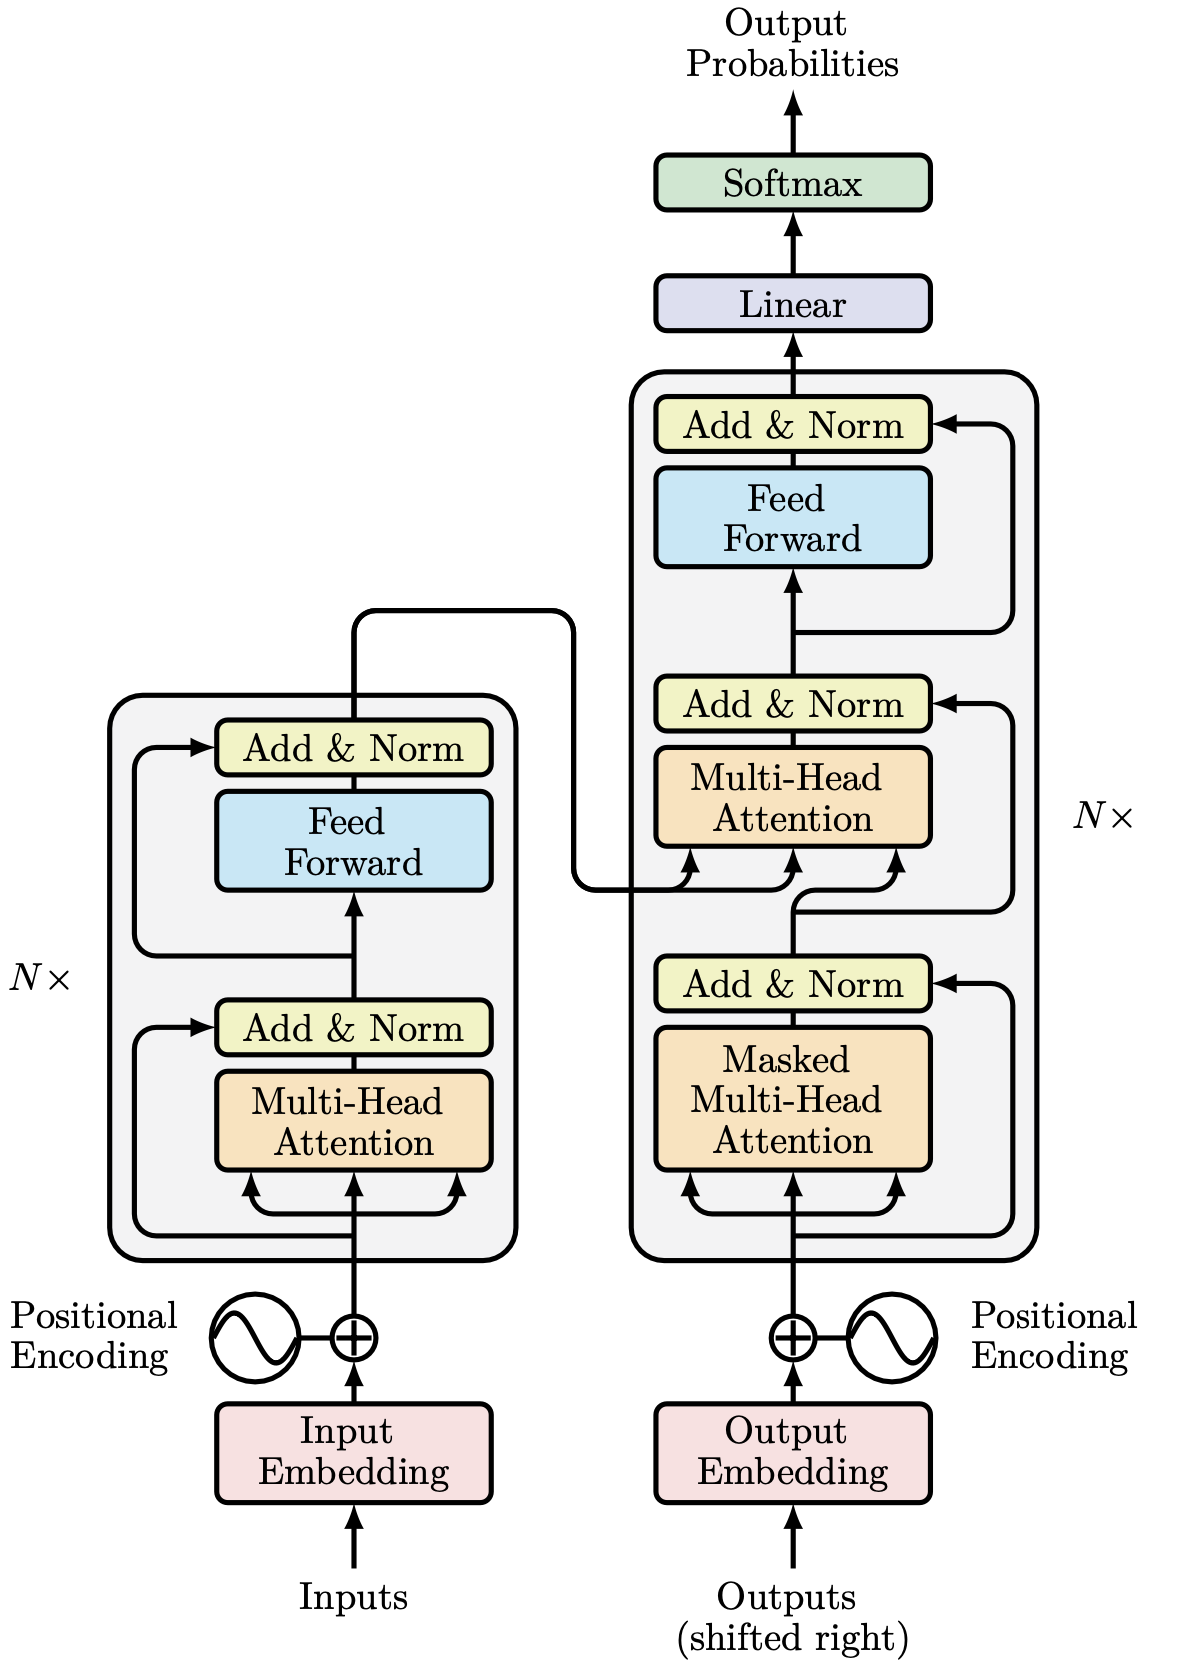
\includegraphics[width=0.6\textwidth]{transformer-arch}
    \caption{Архитектура трансформера}
    \label{fig:transformer-arch}
\end{figure}


\subsection{МЕХАНИЗМ ВНИМАНИЯ В ТРАНСФОРМЕРАХ}
PLACEHOLDER

\subsection{МОДЕЛЬ T5: АРХИТЕКТУРА И ЕЕ ОСОБЕННОСТИ}
PLACEHOLDER

\subsection{FLAN}
PLACEHOLDER
